%!TEX root = FreeRtos ARM uController.tex
\subsection{Scheduling}
\label{Scheduling}
%Ich hab im Duden nachgeschlagen, es heißt wohl der Task. Ich versuche das im ganzen Dokument glatt zu ziehen
%Michael: Ok
Der Scheduler ist die Kernkomponente eines Echtzeitbetriebssystem Kernels, da er eine quasi parallele Aus\-füh\-rung von Tasks ermöglicht. Ein Task stellt dabei eine ei\-gen\-stän\-di\-ge lauffähige Programmeinheit dar. Gewöhnlich implementiert ein Task eine endlose Schleife, die bis zur ihrer Ausführung auf ein Timingevent oder ein Synchronisierungsevent blockiert (Listing \ref{lst:taskPseudo}). Die einmalige Aus\-füh\-rung eines Tasks wird Job\cite{9780128015070} genannt. 
\begin{lstlisting}[caption={Pseudocode für die Implementierungsmuster eines periodischen (zeitgesteuert) Tasks und sporadischen (eventgesteuert) Tasks ~\protect\citeA{LorenK.Rhodes2017}}, linewidth=8cm,captionpos=b, label=lst:taskPseudo, float=hbt]
//Periodische Task
while(true)
{
   waitForStartOfNextCycle; //the period is p msec
   ExecProcess();  //takes c msec in the worst case
}

//Sporadische Task
while(true)
{
   waitForEvent;   //successive events won't occur in less than p msec
   ExecResponseProcess();   //takes c msec worst case
}
\end{lstlisting}
Abhängig vom aktuellen Zustand aller Tasks und dem gewählten Scheduling\-algorithmus wählt der Scheduler den nächsten Task, der ausgeführt werden soll. Auf einem $\mu$Controller mit einem Kern (Prozessoreinheit) kann dabei immer nur ein Task ausgeführt werden. Die Ausführung ist also nicht wirklich parallel, sondern eine sequentielles Ausführen von Task Jobs, die durch den Scheduler organisiert werden. Der Vorgang des Task-Wechsels durch den Scheduler wird Kontextwechsel oder Contextswitch genannt. Der Kontextwechsel beeinflusst die Instruktionsfolge des Tasks nicht. Zum Zeitpunkt der Unterbrechung wird durch den Scheduler eine Art Schnappschuss des Tasks erstellt. Alle Register und der Stack des Tasks werden gesichert. Nachdem der Scheduler den verdrängten Task wieder zur Aus\-füh\-rung ausgewählt hat, werden alle Register und der Stack wiederhergestellt und in die entsprechenden $\mu$\-Pro\-zes\-sor\-re\-gis\-ter geladen. Der Task wird danach ab der letzten Instruktion fortgeführt. Abbildung \ref{fig:ContextSwitch} zeigt wie ein Task wäh\-rend seiner Ausführung unterbrochen wird.
%Michael in einer Zeiteinheit habe ich wieder entfernt, da es das ganze mit Timeslicing und Tick interrupts durcheinader bringt. 
\begin{figure}[ht!]
	\centering
		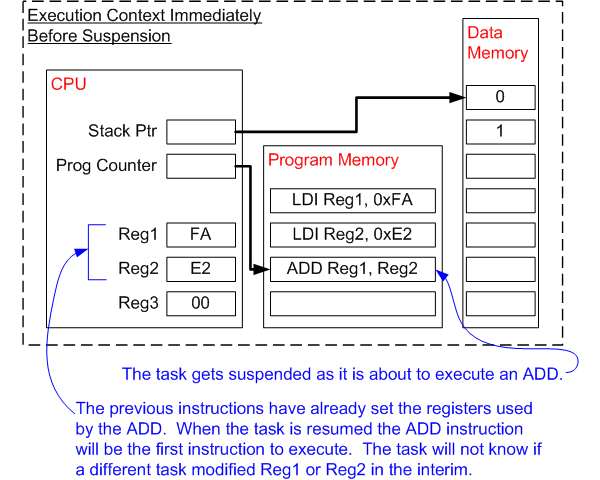
\includegraphics[width=0.4\textwidth]{Pictures/FreeRTOSOrg/ExeContext.png}
	\caption{Der Kontextwechsel eines Tasks findet mitten in der Aus\-füh\-rung statt. Alle Register, die für die weitere Ausführung benötigt werden, werden durch den Scheduler gesichert. Bild-Quelle~\protect\citeA{MasteringFreeRtos} }
	\label{fig:ContextSwitch}
\end{figure}
\newline
Neben den User-Tasks, die durch den Entwickler erstellt werden, gibt es noch den Idle Task. Dieser wird automatisch beim Start des Schedulers erstellt. Der Idle Task hat immer die niedrigste Priorität (0) und wird immer dann ausgeführt, wenn kein User-Task zur Aus\-füh\-rung bereit steht. Der Idle Task ist ein Indikator für über\-schüss\-ige Prozessorzeit. Mittels der Idle-Hook Funktion kann dem Idle Task Funktionalität durch den Entwickler hinzugefügt werden. Wie der Idle Task zum Energiesparen genutzt werden kann wird in Abschnitt \ref{sec:Low Power Modes} beschrieben.
Folgende Zu\-stän\-de kann ein FreeRTOS Task im Scheduling annehmen: 
\begin{itemize}
	\item Running: Der Task wird zur Zeit vom Scheduler ausgeführt.
	\item Blocked: Der Task ist nicht bereit und wartet auf ein Synchronisations- oder ein Timer Event.
	\item Ready: Der Task ist bereit und wartet auf seine Aus\-füh\-rung durch den Scheduler.
	\item Suspended: Der Task hat vTaskSuspend() aufgerufen und wurde vom Schedulingvorgang ausgeschlossen.
\end{itemize}
 Abbildung \ref{fig:TaskStates} zeigt ein vollständiges Zustandsdiagramm eines FreeRTOS Tasks.
\begin{figure}[ht!]
	\centering
		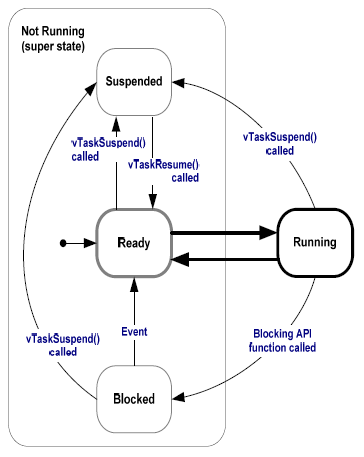
\includegraphics[width=0.2\textwidth]{Pictures/FreeRTOSOrg/taskStates.png}
	\caption{Übersicht aller Task-Zustandstransitionen in FreeRTOS. Der Zustandswechsel findet entweder durch den Aufruf einer FreeRTOS API Funktion statt oder aber durch Events (z.B. Interrupts, Timer-Events). Der Wechsel in den Zustand Running wird durch den Scheduler bestimmt und ist durch den Schedulingalgorithmus definiert.  Bild-Quelle~\protect\citeA{MasteringFreeRtos}}
	\label{fig:TaskStates}
\end{figure} 
\newline
Die Grundlage aller zur Verfügung stehenden Scheduling\-algorithmen ist das Round Robin Verfahren\cite{9783827373427}. Dabei werden alle lauf\-fäh\-igen Tasks (Ready) gleicher Priorität in einer Liste verwaltet. Jeder Task in der Liste erhält ein gewisses Zeitquantum\footnote{Round Robin definiert nicht die Länge des Zeitquantums}, welches bestimmt, wie lange einem Task der Prozessor zugeteilt wird. Nach Ablauf des Zeitquantums wird ein Kontextwechsel durchgeführt. Der näch\-ste Task in der Liste erhält Prozessorzeit und der ausgelaufene Task wird durch den Scheduler automatisch hinten an die Liste angefügt. Da jedem Task in FreeRTOS eine gewisse Priorität zugewiesen wird, ist auch für jede Priorität eine eigene Round Robin-Liste nötig. Dieses Verfahren wird auch Priority Scheduling \cite{9783827373427} genannt. Abbildung \ref{fig:PrioList1} veranschaulicht den Aufbau dieser Listen und in Listing \ref{lst:nextTask} wird gezeigt wie das Priority Scheduling im FreeRTOS Source Code umgesetzt wird. 
\begin{figure}[htb]
	\centering
		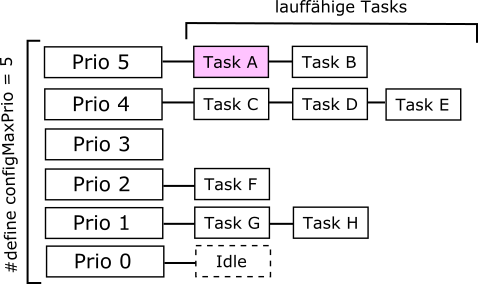
\includegraphics[width=0.3\textwidth]{Pictures/Scheduling/PrioList1.png}
	\caption{Aufbau der Prioritätenliste nach Round Robin in FreeRTOS. Alle aufgeführten Tasks sind bereit zur Ausführung. Task A wird aktuell durch den Scheduler ausgeführt. Nach dem Ablauf des Zeitquantums wird A hinter B einsortiert. Die Maximale Priorität wird durch configMaxPrio bestimmt. Der Idle Task wird automatisch durch den Kernel erzeugt und hat immer die niedrigste Priorität. }
	\label{fig:PrioList1}
\end{figure}
\begin{lstlisting}[caption={FreeRTOS Source zur Priroty Task Selection aus Task.c. Alle lauffähigen Tasks werden in einem Array verwaltet pxReadyTaskLists. Die Listen verwalten sich durch Referenz-Pointer in den TCBs der einzelnen Tasks.}, linewidth=8cm,captionpos=b, label=lst:nextTask, float=hbt]
#define taskSELECT_HIGHEST_PRIORITY_TASK(){																									
	UBaseType_t uxTopPriority = uxTopReadyPriority;														
		/* Find the highest priority queue that contains ready tasks. */								
		while(listLIST_IS_EMPTY(&(pxReadyTasksLists[ uxTopPriority ]))){																								
			configASSERT( uxTopPriority );																
			--uxTopPriority;																			
		}																								
		/* listGET_OWNER_OF_NEXT_ENTRY indexes through the list, so the tasks of						
		the	same priority get an equal share of the processor time. */									
		listGET_OWNER_OF_NEXT_ENTRY(pxCurrentTCB, &(pxReadyTasksLists[uxTopPriority]));			
		uxTopReadyPriority = uxTopPriority;																
	} /* taskSELECT_HIGHEST_PRIORITY_TASK */
\end{lstlisting}
Dem Entwickler stehen zwei Konfigurationsmöglichkeiten des FreeRTOS Scheduler zur Auswahl: Der Scheduler kann entweder im Cooperative Mode oder im Preemptive Mode ausgeführt werden. Welchen Modus der Scheduler als Schedulingalgorithmus verwendet, wird durch das folgende Define in der FreeRTOS config bestimmt:
\begin{lstlisting}[numbers = none]
#define configUSE_PREEMPTION
\end{lstlisting}
Im Preemptive Mode wird ein aktiver Task mit niedriger Priorität sofort von einem Task mit höherer Priorität verdrängt. Ein Kontextwechsel wird durchgeführt. Im Cooperative Mode hingegen wird ein Kontextwechsel erst durchgeführt, wenn ein Task den Prozessor explizit abgibt. Dies geschieht beispielsweise durch die Funktion xTaskYield() oder durch einen blockierenden API Aufruf. Abbildung \ref{fig:PreVSCo} zeigt den Vergleich beider Modi durch einen beispielhaften Ablauf. 
\begin{figure}[htb]
	\centering
		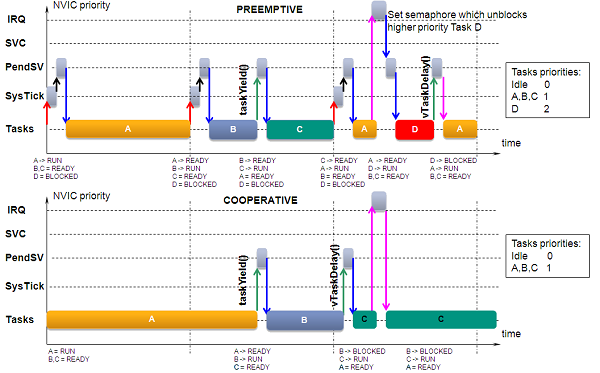
\includegraphics[width=0.4\textwidth]{Pictures/EMCUIT/PreemptiveCooperative.png}
	\caption{Im Cooperative Mode wird der Prozessor von einem Task erst abgegeben, wenn dieser explizit taskYield() aufruft. Selbst wenn ein Task mit höherer Priorität in den Ready Zustand wechselt, läuft der Task mit niedrigerer Priorität weiter. Im Gegensatz dazu steht das Pre-Emptive Scheduling (hier mit Time-Slicing). Es unterbricht den laufenden Task mit niedrigerer Priorität sofort, sobald ein Task mit höherer Priorität in den Zustand Ready wechselt. Bild-Quelle~\protect\citeA{MasteringFreeRtos}}
	\label{fig:PreVSCo}
\end{figure}
Für den Preemptive Mode bietet FreeRTOS eine weitere Konfigurationsmöglichkeit. Mit der nachfolgenden Pre-Prozessordirektive lässt sich das Zeitschlitzverfahren (time slicing) aktivieren: 
\begin{lstlisting}[numbers = none]
#define configUSE_TIME_SLICING 1
\end{lstlisting}
Durch das Zeitschlitzverfahren wird die zugeteilte Prozessorzeit für Tasks gleicher Priorität gleichmäßig aufgeteilt. Dies geschieht durch Ein\-füh\-rung eines festen Tick-Interrupt Intervalls. Bei jedem Tick-Interrupt wird der FreeRTOS SysTickHandler aufgerufen. Listing \ref{lst:SysTickS} zeigt die Implementierung des FreeRTOS SysTicks. Der SysTickHandler ist Bestandteil des Schedulers. Er überprüft bei jeder Ausführung, ob sich ein Task gleicher Priorität im Ready Zustand befindet. Sollte es einen solchen Task geben, wird ein Kontextwechsel durchgeführt und der Task bekommt den Prozessor zugeteilt. Des Weiteren kümmert sich der SysTickHandler um die Verwaltung des TickCounts, welcher als Referenz für alle RTOS Timingfunktionen dient. Abbildung \ref{fig:SysTick} zeigt diesen Vorgang im zeitlichen Verlauf.
\begin{lstlisting}[caption={FreeRTOS Source des SysTickHandlers aus Task.c. Der SysTickHandler verwaltet den TickCount. Der TickCount dient allen Timingfunktionen des RTOS Kernels als Zeitreferenz. Des Weiteren wird beim aktiven Time Slicing überprüft, ob ein Kontextwechsel nötig ist. Der Kontextwechsel wird dann ggf. durch den PendSVHandler durchgeführt.}, linewidth=8cm,captionpos=b, label=lst:SysTickS, float=hbt]
void xPortSysTickHandler( void ){
	portDISABLE_INTERRUPTS();
	{
		/* Increment the RTOS tick. */
		if( xTaskIncrementTick() != pdFALSE )
		{
			/* A context switch is required. */
			portNVIC_INT_CTRL_REG = portNVIC_PENDSVSET_BIT;
		}
	}
	portENABLE_INTERRUPTS();
}
\end{lstlisting}
\begin{figure}[htb]
	\centering
		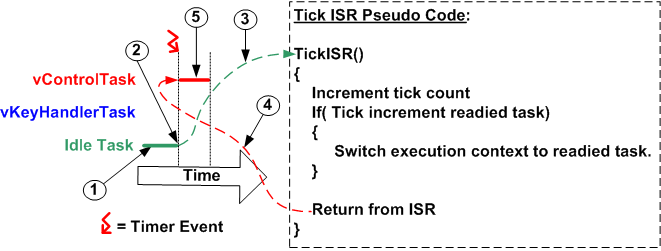
\includegraphics[width=0.4\textwidth]{Pictures/FreeRTOSOrg/TickISR.png}
	\caption{Beispielhafter Ablauf eines SysTickInterrupts.(1) kein User Task ist ready, der Idle Task ist aktiv. (2) SysTickInterrupt. (3) SysTickHandler wird aufgerufen. (4) vControlTask ist ready und ein Kontextwechsel wird durchgeführt. vControlTask hat hier die gleiche Priorität wie der IdleTask. (5)vControlTask wird ausgeführt. Bild-Quelle~\protect\citeA{MasteringFreeRtos}}
	\label{fig:SysTick}
\end{figure}
Die wahrscheinlich am häufigsten verwendete Konfiguration ist der Preemptive Mode mit aktivem Zeitschlitzverfahren:
\begin{lstlisting}[numbers = none]
#define configUSE_PREEMPTION 1
#define configUSE_TIME_SLICING 1
\end{lstlisting}
Diese Einstellung wird üblicherweise Prioritized Pre-emptive Scheduling with Time Slicing genannt. Abbildung \ref{fig:timeslice} zeigt wie sich diese Konfiguration des Schedulers bei mehreren Tasks mit unterschiedlicher Priorität verhält.
\begin{figure}[htb]
	\centering
		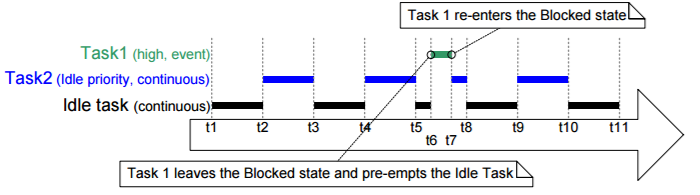
\includegraphics[width=0.5\textwidth]{Pictures/Scheduling/timeslice2.png}
	\caption{Durch das Zeitschlitzverfahren wechseln sich Task1 und Idle Task bei jedem SysTick Interrupt ab, da beide die gleiche Priorität haben. Bei T6 ist Task 1 bereit und verdrängt (preempt) aufgrund seiner höheren Priorität Task2. Nachdem Task 1 blockiert, wird Task 2 fortgeführt. Bild-Quelle~\protect\citeA{MasteringFreeRtos}}
	\label{fig:timeslice}
\end{figure}
\subsection{Echtzeitfähigkeit}
%---------------------------------------Work in Progress--------------------------------------
Ein Echtzeitbetriebssystem zeichnet sich dadurch aus, dass es auf ein eintreffendes Ereignis eine deterministische und somit vorhersehbare Reaktion gibt. Dies wird bei FreeRTOS, wie bei allen anderen Echtzeitbetriebssystemen unter anderem durch geeignete Scheduling Stategien und nicht blockierende Interprozesskommunikation erreicht\cite{9780128015070} \cite{Jones:1997:CRT:269005.266689} \cite{Regehr:2001:ACR:882481.883779}. In FreeRTOS wird beispielsweise fixed priorty preemtive Scheduling als Schedulerstrategie verwendet. Bei prioritätenbasierenden Verfahren erhalten Task mit Echtzeitanforderung (Echtzeittask) eine höhere Priorität als Tasks ohne Echtzeitanforderungen. So kann garantiert werden, dass ein Echtzeittask nicht von einem Task ohne Echtzeitanforderungen blockiert wird. Durch die Zuweisung einer höheren Priorität ist aber noch nicht sichergestellt, dass der Echtzeittask die geforderten Deadlines einhält. Sind mehrere Echtzeittasks in einer Anwendung vorhanden, kann eine unpassende Prioritätenzuweisung dazu füh\-ren, dass die Anwendung ihre Deadlines nicht einhalten kann\cite{9780128015070}. Ob die gesamte Anwendung theoretisch "`schedulbar"' , d.h. ob alle geforderten Deadlines und Perioden eingehalten werden, wird gewöhnlich zu Beginn einer Entwicklung (Designphase) in einer Schedulinganalyse bestimmt. Die Schedulinganalyse umfasst unter anderem die Bestimmung von worst case runtimes und worst case response times der Tasks, sowie die Festlegung der Prioritäten durch spezielle Verfahren, wie rate monotonic assignment (RMA) oder deadline monotonic assignment (DMA). Eine sehr gute Beschreibung zur Scheduling Analyse und den Verfahren zur Prioritätenvergabe finden sich in \cite{9780128015070}.
FreeRTOS bietet alle Techniken, die für die Implementierung von Echtzeitsystem benötigt werden, daher kann man sagen, dass FreeRTOS für weiche Echtzeitsysteme geeignet ist. 
Bei harten Echtzeitanforderungen hängt dies stark vom Kontext der Zielanwendung ab. In harten Echtzeitsystemen ist die Performance des Schedulers (Ein/Auslagern einer Task) und der API Funktionen ebenfalls zu berücksichtigen, diese werde aber von Real Time Engineers nicht veröffentlicht. Um zu gewährleisten das ein Echtzeitanwendung mit FreeRTOS harten Echtzeitanforderungen genügt, muss durch Echtzeit Performance Messungen bestimmt werden \cite{RealTimePerformance}.  

